\documentclass[12pt,xcolor={usenames,dvipsnames,x11names}]{beamer}
\usepackage{style/style}
\setbool{writein}{true}

%-----------------
% Slides
%-----------------
\begin{document}

% Title Slide
{
\setbeamercolor{background canvas}{bg=eblue}
\begin{frame}[b,plain]
\phantom{.}\par
\phantom{.}\hfill{\Large\color{egold} Lecture $\pi$-Day:} \hfill\phantom{.}\pvspace{0.1cm}
\phantom{.}\hfill{\Large\color{egold} Polar Form of\; \hfill \phantom{.} \par\vspace{0.1cm} \phantom{.} \hfill Complex Numbers} \hfill \phantom{.} \pvspace{0.2cm}
\makebox[\linewidth]{\includegraphics[width=1.4\paperwidth]{images/fgcu.jpeg}}
\end{frame}
}



% Things to Review
\begin{frame}[plain] \frametitle{Things to Review:}
\begin{itemize} \itemsep=3ex
\item Complex Arithmetic:
	\begin{enumerate}[--]
	\item \href{https://www.youtube.com/watch?v=OQz1ydBcQSA}{The Organic Chemistry Tutor}
	\item \href{https://www.youtube.com/watch?v=5PcpBw5Hbwo}{3Blue1Brown}
	\item \href{https://www.youtube.com/watch?v=wQnXN0xljR0}{The A+ Tutor}
	\item \href{https://www.youtube.com/watch?v=ysVcAYo7UPI&list=PLXSlB4yMaoJtM2gG5Mas5mMjwX_B51vsB}{Khan Academy}
	\end{enumerate}

\item Unit Circle \& Trig. Values:
	\begin{enumerate}[--]
	\item \href{https://www.youtube.com/watch?v=V5ArB_GFGYQ}{The Organic Chemistry Tutor}
	\item \href{https://www.youtube.com/watch?v=3KYomDEIQgo}{Maths Genie}
	\item \href{https://www.youtube.com/watch?v=1m9p9iubMLU&list=PLSQl0a2vh4HDEMO_W3DWpSgfHIF6AKDz1}{Khan Academy}
	\item \href{https://www.youtube.com/watch?v=75dMcyCUo2g}{Professor Dave Explains}
	\end{enumerate}
\end{itemize}
\end{frame}



% You Should Be Able To...
\begin{frame}[plain] \frametitle{You Should Be Able To\dots}
\fontsmall
\begin{itemize} \itemsep=3ex
\item Define the absolute value/modulus of a complex number
\item Compute the absolute value of a complex number.
\item Define and find the argument of a complex number.
\item Define the rectangular and polar form of a complex number.
\item Find the polar form of a complex number.
\item Find the rectangular form of a complex number.
\item State DeMoivre's Theorem.
\item Use DeMoivre's Theorem to find powers and roots of complex numbers.
\end{itemize}
\end{frame}



% Recalling Complex Arithmetic
\begin{frame}[t] \frametitle{Recalling Complex Arithmetic} 
{\small You have seen how to perform arithmetic with complex numbers, i.e. numbers of the form $a + bi$:}

\begin{myex} 
\color{white}
	\textbullet\ {\small \itshape Addition:} \scalebox{0.9}{$(3 - 4i) + (2 + i)= (3 + 2) + (-4 + 1)i= 5 - 3i$} \par\vspace{0.6cm}
	\textbullet\ {\small \itshape Subtraction:} \scalebox{0.9}{$(5 - i) - (1 - 4i)= (5 - 1) + \big(-i - (-4) \big)\, i= 4 + 3i$} \par \vspace{0.6cm}
	\textbullet\ {\small \itshape Multiplication:} \scalebox{0.75}{$(2 - i)(1 + 4i)= 2 + 8i - i - 4i^2= 2 + 7i - 4(-1)= 6 + 7i$} \par \vspace{0.6cm}
	\textbullet\ {\small \itshape Division:} \par\vspace{0.2cm} \scalebox{0.85}{$\dfrac{20 + 10i}{3 + 4i}= \dfrac{20 + 10i}{3 + 4i} \cdot \dfrac{3 - 4i}{3 - 4i}= \dfrac{(20 + 10i)(3 - 4i)}{3^2 + 4^2}= \dfrac{100 - 50i}{25}= 4 - 2i$} \par \vspace{0.6cm}
	\textbullet\ {\small \itshape Powers:} \scalebox{0.90}{$(2 + i)^3= (2 + i)(2 + i)(2 + i)= (3 + 4i)(2 + i)= 2 + 11i$}
\end{myex}

\end{frame}



% Absolute Value
\begin{frame}[t] \frametitle{Absolute Value/Modulus}

{\small The {\itshape absolute value/modulus} of a complex number $z= a + bi$ is\dots
	\[
	|z|:= \sqrt{a^2 + b^2}
	\]
}

	\begin{minipage}{0.49\textwidth}
	\[
	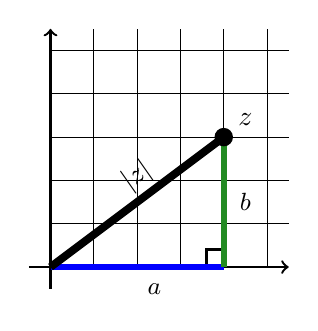
\begin{tikzpicture}[scale=0.55]
	\draw[line width=0.03cm,->] (0,-0.5) -- (0,5.5);
	\draw[line width=0.03cm,->] (-0.5,0) -- (5.5,0);
	\foreach \x in {1,2,...,5}
		{
		\draw[line width=0.01cm] (\x,0) -- (\x,5.5);
		%\node at (\x,-0.25) {\tiny$\x$};
		}
	\foreach \y in {1,2,...,5}
		{
		\draw[line width=0.01cm] (0,\y) -- (5.5,\y);
		%\node at (-0.25,\y) {\tiny$\y$};
		}
	% Angle
	\draw[line width=0.04cm] (3.6,0) -- (3.6,0.4) -- (4,0.4);
	% Sides
	\draw[line width=0.08cm,blue] (0,0) -- (4,0);
	\draw[line width=0.08cm,ForestGreen] (4,0) -- (4,3);
	% Ray
	\draw[line width=0.1cm] (0,0) -- (4,3);
	\draw[fill=black] (4,3) circle (0.2);
	% x, y
	\node at (2.4,-0.5) {\small$a$};
	\node at (4.5,1.5) {\small$b$};
	\node at (4.5,3.4) {$z$};
	\node[rotate=35] at (2,2.1) {$|z|$};  
	\end{tikzpicture}
	\]	
	\end{minipage}	\begin{minipage}{0.49\textwidth}
	{\footnotesize Imagine plotting the complex number $z= a + bi$. \par\vspace{0.3cm}
	
	The absolute value of $z$ is simply the length of the line segment connecting $z$ to the origin.
	}
	\end{minipage} 



% Example
\begin{myex}
\color{white} \small If $z= 1 - 4i$, then\dots
	\[
	|z|= \sqrt{1^2 + (-4)^2}= \sqrt{1 + 16}= \sqrt{17} \approx 4.12311
	\]
\end{myex}
\end{frame}



% Try It!
\begin{frame}[t] \frametitle{Try It!}
{\small Let $z= -3 + 4i$. Plot the complex number $z$ and compute $|z|$.}
\end{frame}



% Deriving the Polar Form
\begin{frame}[t] \frametitle{Deriving the Polar Form}

{\footnotesize Imagine plotting the complex number $z= a + bi$.}

	% Side-by-Side
	\begin{minipage}{0.49\textwidth} % LEFT SIDE
	\[
	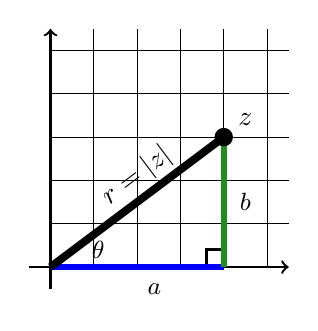
\begin{tikzpicture}[scale=0.55]
	\draw[line width=0.03cm,->] (0,-0.5) -- (0,5.5);
	\draw[line width=0.03cm,->] (-0.5,0) -- (5.5,0);
	\foreach \x in {1,2,...,5}
		{
		\draw[line width=0.01cm] (\x,0) -- (\x,5.5);
		%\node at (\x,-0.25) {\tiny$\x$};
		}
	\foreach \y in {1,2,...,5}
		{
		\draw[line width=0.01cm] (0,\y) -- (5.5,\y);
		%\node at (-0.25,\y) {\tiny$\y$};
		}
	% Angle
	\draw[line width=0.04cm] (3.6,0) -- (3.6,0.4) -- (4,0.4);
	% Sides
	\draw[line width=0.08cm,blue] (0,0) -- (4,0);
	\draw[line width=0.08cm,ForestGreen] (4,0) -- (4,3);
	% Ray
	\draw[line width=0.1cm] (0,0) -- (4,3);
	\draw[fill=black] (4,3) circle (0.2);
	% x, y
	\node at (2.4,-0.5) {\small$a$};
	\node at (4.5,1.5) {\small$b$};
	\node at (4.5,3.4) {$z$};
	\node[rotate=37] at (2,2.1) {$r= |z|$};  
	% Angle
	\node at (1.1,0.4) {\small$\theta$};
	\end{tikzpicture}
	\]	
	\end{minipage}	\begin{minipage}{0.49\textwidth} % RIGHT SIDE
	{\footnotesize We know that $z= a + bi$. But using right-triangle trig:
		\[
		\begin{aligned}
		\cos \theta= \dfrac{a}{r} \quad\Longrightarrow\quad a = r \cos \theta \\
		\sin \theta= \dfrac{b}{r} \quad\Longrightarrow\quad b = r \sin \theta \\
		\end{aligned}
		\]
	}
	\end{minipage} \par\vspace{0.3cm}

% Bottom Text
{\footnotesize But then $z= x + yi= r \cos \theta + i(r \sin \theta) \,i= r \, (\cos \theta + i \sin \theta)$. This is the \textit{polar representation} of $z$ and the angle $\theta$ is called the \textit{argument} of $z$.}

\begin{mydef}[Polar Form]
\color{egold} \small Given the \textit{rectangular form} $z= a + bi$, the polar form of $z$ is\dots
	\[
	z= r \,(\cos \theta + i \sin \theta)
	\]
\end{mydef}
\end{frame}



% Example
\begin{frame}[t] \frametitle{Example}
{\small Find the polar representation of $z= -3 + 4i$.}
\end{frame}



% Try It!
\begin{frame}[t] \frametitle{Try It!}
{\small Find the polar representation of $5 - 5i$.}
\end{frame}



% Example
\begin{frame}[t] \frametitle{Example}
{\footnotesize Find the rectangular representation of $z= 10 \left( \cos \left(\tfrac{5\pi}{6} \right) + i \sin \left( \tfrac{5\pi}{6} \right) \right)$.}
\end{frame}



% Try It!
\begin{frame}[t] \frametitle{Try It!}
{\footnotesize Find the rectangular representation of $3 \,\big( \cos(330^\circ) + i \sin(330^\circ) \big)$.}
\end{frame}



% DeMoivre's Theorem
\begin{frame}[t]
\phantom{.}\vfill \begin{center} \bfseries \LARGE \color{eblue} De Moivre's Theorem \end{center} \vfill
\end{frame}



% Absolute Value
\begin{frame}[t] \frametitle{De Moivre's Theorem}
\footnotesize De Moivre's Theorem allows one to compute powers of complex numbers easily.  

\begin{mythm}[De Moivre's Theorem]
\color{egold} If $z= a + bi$, has polar form $z= r \,(\cos \theta + i \sin \theta)$ then\dots
	\[
	z^n= r^n \, \big( \cos(n\theta) + i \sin(n \theta) \big)
	\]
\end{mythm} \par\vspace{0.3cm}

{\itshape \color{egreen} \bfseries Computing Complex Powers:} To compute a power of a complex number $z$, say $z^n$, you need to\dots
	\begin{enumerate}[1.]
	\item Find the polar form of $z$.
	\item Use De Moivre's Theorem to write 
		\[
		z^n= r^n \, \big( \cos(n\theta) + i \sin(n \theta) \big)
		\]
	That is, compute the $n$th power of its absolute value and multiply the angle by $n$.
	\item Simplify this expression (if possible).
	\end{enumerate}
\end{frame}



% Example
\begin{frame}[t] \frametitle{Example}
{\small\itshape Compute $(-2 + 4i)^4$.} \par\vspace{0.5cm}

\end{frame}



% Try It!
\begin{frame}[t] \frametitle{Try It!}
{\footnotesize If $z= 5 - 5i$, compute $z^3$.}
\end{frame}



% Roots of Complex Numbers
\begin{frame}[t]
\phantom{.}\vfill \begin{center} \bfseries \LARGE \color{eblue} Roots of Complex Numbers \end{center} \vfill
\end{frame}



% Complex Roots
\begin{frame}[t] \frametitle{De Moivre's Theorem}
\scriptsize De Moivre's Theorem also allows one to compute roots of complex numbers `easily.' \par\vspace{0.3cm}

But just like $\sqrt{4}= \pm 2$, i.e. $4$ has two possible square roots, there will be $n$ possible $n$th roots for a complex number.

\begin{mythm}[De Moivre's Theorem]
\footnotesize\color{egold} If $z= a + bi$, has polar form $z= r \,(\cos \theta + i \sin \theta)$ then\dots
	\[
	\begin{aligned}
	\underbrace{\sqrt[n]{z}}_{\text{Or } z^{1/n}}&= \sqrt[n]{r} \, \left( \cos \left( \dfrac{\theta + 2\pi k}{n} \right) + i \sin \left( \dfrac{\theta + 2\pi k}{n} \right) \right) & \qquad \text{(radians)} \\[0.5cm]
	\underbrace{\sqrt[n]{z}}_{\text{Or } z^{1/n}}&= \sqrt[n]{r} \, \left( \cos \left( \dfrac{\theta + 360^\circ k}{n} \right) + i \sin \left( \dfrac{\theta + 360^\circ k}{n} \right) \right) & \text{(degrees)}
	\end{aligned}
	\]
where $k= 0, 1, 2, \ldots, n-1$.
\end{mythm} \par\vspace{0.4cm}

{\scriptsize\textit{Note.} This says the complex $n$th roots of $z$ are equally spaced points on the circle at the origin with radius $\sqrt[n]{z}$---each $\frac{360^\circ}{n}$ degrees apart.}
\end{frame}



% Complex Roots
\begin{frame}[t] \frametitle{Computing Complex Roots}

\begin{mythm}[De Moivre's Theorem] 
\scriptsize\color{egold} If $z= a + bi$, has polar form $z= r \,(\cos \theta + i \sin \theta)$ then\dots
	\[
	\begin{aligned}
	\underbrace{\sqrt[n]{z}}_{\text{Or } z^{1/n}}&= \sqrt[n]{r} \, \left( \cos \left( \dfrac{\theta + 2\pi k}{n} \right) + i \sin \left( \dfrac{\theta + 2\pi k}{n} \right) \right) & \qquad \text{(radians)} \\[0.5cm]
	\underbrace{\sqrt[n]{z}}_{\text{Or } z^{1/n}}&= \sqrt[n]{r} \, \left( \cos \left( \dfrac{\theta + 360^\circ k}{n} \right) + i \sin \left( \dfrac{\theta + 360^\circ k}{n} \right) \right) & \text{(degrees)}
	\end{aligned}
	\]
where $k= 0, 1, 2, \ldots, n-1$.
\end{mythm} \par\vspace{0.2cm}

{\scriptsize\itshape \color{egreen} \bfseries Computing Complex Roots:} \scriptsize To compute the $n$th roots of a complex number $z$, say $\sqrt[n]{z}$, you need to\dots
	\begin{enumerate}[1.]
	\item Find the polar form of $z$.
	\item Use De Moivre's Theorem to write 
		\[
		\sqrt[n]{z}= \sqrt[n]{r} \, \big( \cos(n\theta) + i \sin(n \theta) \big)
		\]
	That is, compute the $n$th root of its absolute value, divide the angle by $n$, and write out each possible root by plugging in $k= 0, 1, \ldots, n - 1$.
	\item Simplify these expressions (if possible).
	\end{enumerate}
\end{frame}



% Example
\begin{frame}[t] \frametitle{Example}
{\footnotesize Find all the complex cube roots of $-1= 1 \big( \cos 180^\circ + i \sin 180^\circ \big)$.}
\end{frame}



% Try It!
\begin{frame}[t] \frametitle{Try It!}
{\footnotesize Find all the complex fourth roots of $16 \big( \cos 120^\circ + i \sin 120^\circ \big)$.}
\end{frame}



% Extra Facts
\begin{frame}[t]
\phantom{.}\vfill \begin{center} \bfseries \LARGE \color{eblue} Extra Facts \end{center} \vfill
\end{frame}



% Euler's Identity
\begin{frame}[t] \frametitle{Euler's Identity}
\footnotesize All of this is related to Euler's Identity:

\begin{mythm}[\small Euler's Identity]
\color{egold} \vspace{-0.3cm}
	\[
	e^{i\theta}= \cos \theta + i \sin \theta
	\]
\end{mythm} \par\vspace{0.3cm}

This leads to one of the most famous identities of all time:
	\[
	\begin{aligned}
	e^{i \pi}= \cos(\pi) + i \sin(\pi)= -1 + i(0)= -1
	\end{aligned}
	\]
But then adding 1 to both sides, we have\dots
	\[
	e^{i \pi} + 1= 0
	\]
This has nearly every `important' constant all in one equation: $1, 0, \pi, e,$ and $i$! \par\vspace{0.3cm}

{\footnotesize This allows allows one to write the polar form of a complex number $z$ as\dots
	\[
	z= x + iy= r \,(\cos \theta + i \sin \theta)= r e^{i\theta}
	\]
}
\end{frame}



% Computing with the Alternative Polar Form
\begin{frame}[t] \frametitle{\large Computing with the Alternative Polar Form}

\footnotesize Using the polar form $z= r e^{i \theta}$, we can perform complex multiplication, division, and powers quite easily! \par\vspace{0.3cm}

{\footnotesize\color{eblue} \bfseries Example.} Let $z= -\sqrt{3} + i$ and $w= 3 + 3 \sqrt{3} i$. \par\vspace{0.3cm}

One can find (\textit{Try It!}) that $z$ and $w$ have polar forms\dots
	\[
	\begin{aligned}
	z&= 6 \, \left( \cos \left( \tfrac{\pi}{3} \right) + i \sin \left( \tfrac{\pi}{3} \right) \right)= 6 e^{i \frac{\pi}{3}} \\[0.1cm]
	w&= 2 \, \left( \cos \left( \tfrac{5\pi}{6} \right) + i \sin \left( \tfrac{5\pi}{6} \right) \right)= 2 e^{i \frac{5\pi}{6}} \\
	\end{aligned}
	\]
But then, for example, we have\dots
	\[
	\begin{aligned}
	\text{\textbullet}\enskip zw&= 6 e^{i \frac{\pi}{3}} \cdot 2 e^{i \frac{5\pi}{6}} \cdot = 12\, e^{i \left( \frac{\pi}{3} + \tfrac{5\pi}{6} \right)}= 12 e^{i \tfrac{7\pi}{6}} \\[0.2cm]
	\text{\textbullet}\enskip \dfrac{z}{w}&= \dfrac{6 e^{i \frac{\pi}{3}}}{2 e^{i \frac{5\pi}{6}}}= 3 e^{i \left( \tfrac{\pi}{3} - \tfrac{5\pi}{6} \right)}= 3 \, e^{-i \frac{\pi}{2}} \\[0.2cm]
	\text{\textbullet}\enskip z^3&= (6 e^{i \frac{\pi}{3}})^3= 6^3 e^{i \frac{\pi}{3} \cdot 3}= 216\, e^{i \pi}
	\end{aligned}
	\]

{\scriptsize \textit{Note.} One can then convert these to their regular representation. For instance, $zw= 12 e^{i \frac{7\pi}{6}}= 12 \big(\cos(\tfrac{7\pi}{6}) + i \sin(\tfrac{7\pi}{6}) \big)= 12 \big(-\tfrac{\sqrt{3}}{2} - i\tfrac{1}{2} \big)= -6 \sqrt{3} - 6i$.}
\end{frame}



% Blank Frame
\begin{frame}[t] \frametitle{} 
\footnotesize Most importantly, now you can understand all them nerd shirts!
	\begin{figure}[!ht]
	\centering
	\includegraphics[width=0.23\textwidth]{images/shirt1.png}
	\includegraphics[width=0.23\textwidth]{images/shirt2.png}
	\includegraphics[width=0.23\textwidth]{images/shirt3.png}
	\includegraphics[width=0.23\textwidth]{images/shirt4.png}
	\end{figure}

Be sure to check out the textbook to see how all this is related to the `mysterious' Mandelbrot set!
	\begin{figure}[!ht]
	\centering
	\includegraphics[width=0.55\textwidth]{images/mandelbrot.jpg}
	\end{figure}	
	
\end{frame}



% Blank Frame
\begin{frame} \frametitle{} \end{frame}

% Blank Frame
\begin{frame} \frametitle{} \end{frame}

% Blank Frame
\begin{frame} \frametitle{} \end{frame}

% Blank Frame
\begin{frame} \frametitle{} \end{frame}

% Blank Frame
\begin{frame} \frametitle{} \end{frame}

% Blank Frame
\begin{frame} \frametitle{} \end{frame}

% Blank Frame
\begin{frame} \frametitle{} \end{frame}

% Blank Frame
\begin{frame} \frametitle{} \end{frame}

% Blank Frame
\begin{frame} \frametitle{} \end{frame}

% Blank Frame
\begin{frame} \frametitle{} \end{frame}

\end{document}


